\documentclass[11pt]{article}

% Language setting
\usepackage[turkish]{babel}
\usepackage{pythonhighlight}

\usepackage[a4paper,top=2cm,bottom=2cm,left=2cm,right=2cm,marginparwidth=2cm]{geometry}

% Useful packages
\usepackage{amsmath}
\usepackage{graphicx}
\usepackage[colorlinks=true, allcolors=blue]{hyperref}
\usepackage{verbatim}
\usepackage{fancyhdr} % for header and footer
\usepackage{titlesec}
\usepackage{parskip}

\setlength{\parindent}{0pt}

\titleformat{\subsection}[runin]{\bfseries}{\thesubsection}{1em}{}

\pagestyle{fancy} % activate the custom header/footer

% define the header/footer contents
\lhead{\small{23BLM-4014 Yapay Sinir Ağları Ara Sınav Soru ve Cevap Kağıdı}}
\rhead{\small{Dr. Ulya Bayram}}
\lfoot{}
\rfoot{}

% remove header/footer on first page
\fancypagestyle{firstpage}{
  \lhead{}
  \rhead{}
  \lfoot{}
  \rfoot{\thepage}
}
 

\title{Çanakkale Onsekiz Mart Üniversitesi, Mühendislik Fakültesi, Bilgisayar Mühendisliği Akademik Dönem 2022-2023\\
Ders: BLM-4014 Yapay Sinir Ağları/Bahar Dönemi\\ 
ARA SINAV SORU VE CEVAP KAĞIDI\\
Dersi Veren Öğretim Elemanı: Dr. Öğretim Üyesi Ulya Bayram}
\author{%
\begin{minipage}{\textwidth}
\raggedright
Öğrenci Adı Soyadı: Cengiz ERMİŞ\\ % Adınızı soyadınızı ve öğrenci numaranızı noktaların yerine yazın
Öğrenci No: 170401019
\end{minipage}%
}

\date{14 Nisan 2023}

\begin{document}
\maketitle

\vspace{-.5in}
\section*{Açıklamalar:}
\begin{itemize}
    \item Vizeyi çözüp, üzerinde aynı sorular, sizin cevaplar ve sonuçlar olan versiyonunu bu formatta PDF olarak, Teams üzerinden açtığım assignment kısmına yüklemeniz gerekiyor. Bu bahsi geçen PDF'i oluşturmak için LaTeX kullandıysanız, tex dosyasının da yer aldığı Github linkini de ödevin en başına (aşağı url olarak) eklerseniz bonus 5 Puan! (Tavsiye: Overleaf)
    \item Çözümlerde ya da çözümlerin kontrolünü yapmada internetten faydalanmak, ChatGPT gibi servisleri kullanmak serbest. Fakat, herkesin çözümü kendi emeğinden oluşmak zorunda. Çözümlerinizi, cevaplarınızı aşağıda belirttiğim tarih ve saate kadar kimseyle paylaşmayınız. 
    \item Kopyayı önlemek için Github repository'lerinizin hiçbirini \textbf{14 Nisan 2023, saat 15:00'a kadar halka açık (public) yapmayınız!} (Assignment son yükleme saati 13:00 ama internet bağlantısı sorunları olabilir diye en fazla ekstra 2 saat daha vaktiniz var. \textbf{Fakat 13:00 - 15:00 arası yüklemelerden -5 puan!}
    \item Ek puan almak için sağlayacağınız tüm Github repository'lerini \textbf{en geç 15 Nisan 2023 15:00'da halka açık (public) yapmış olun linklerden puan alabilmek için!}
    \item \textbf{14 Nisan 2023, saat 15:00'dan sonra gönderilen vizeler değerlendirilmeye alınmayacak, vize notu olarak 0 (sıfır) verilecektir!} Son anda internet bağlantısı gibi sebeplerden sıfır almayı önlemek için assignment kısmından ara ara çözümlerinizi yükleyebilirsiniz yedekleme için. Verilen son tarih/saatte (14 Nisan 2023, saat 15:00) sistemdeki en son yüklü PDF geçerli olacak.
    \item Çözümlerin ve kodların size ait ve özgün olup olmadığını kontrol eden bir algoritma kullanılacaktır. Kopya çektiği belirlenen vizeler otomatikman 0 (sıfır) alacaktır. Bu nedenle çözümlerinizi ve kodlarınızı yukarıda sağladığım gün ve saatlere kadar kimseyle paylaşmayınız.
    \item Bu vizeden alınabilecek en yüksek not 100'dür. Toplam aldığınız puan 100'ü geçerse, aldığınız not 100'e sabitlenecektir.
    \item LaTeX kullanarak PDF oluşturanlar öz geçmişlerine LaTeX bildiklerini de eklemeyi unutmasınlar :)
    \item Bu vizedeki soruların çözümleri ve tex dosyası için istediğiniz kadar sayıda Github repository'si oluşturabilirsiniz. Sadece yukarıda belirttiğim tarihlerde (14 Nisan 2023 saat 15:00 ile 15 Nisan 2023 saat 15:00 arasında) public yapmayı/halka açmayı ve Github profilinizi de öz geçmişinize eklemeyi unutmayın :)
    \item Bilgisayarınıza hiçbir program kurmadan, Overleaf, Google Colab, Kaggle gibi ortamlar üzerinden bu vizeyi tamamlamanız mümkün. İyi çalışmalar!!
\end{itemize}

(Ekstra 5 puan) \url{OdevinTexDosyasınınGithubLinkiniburayakoyun.com}

\newpage
\section{(Toplam 10 Puan) Hopfield Networks:}

\subsection{(2 Puan)} \textbf{ChatGPT’ye size Hopfield Network’ler ile ilgili detaylı bilgi vermesini isteyin. Sorduğunuz soruyu, ChatGPT'nin çıkartığı cevabı aşağı koyun. Bu cevapta anlamadığınız terimleri de ChatGPT’ye sorup, sorduğunuz soruları ve ChatGPT’nin verdiği cevapları da sırayla aşağı koyun.}

SORU1: Hopfield Network'ler ile ilgili detaylı bilgi verirmisin?

Taban olarak sinir ağları alanında kullanılan bir yapay sinir ağı modeli olan Hopfield Ağı (ya da Hopfield Network), birçok alanda uygulama potansiyeline sahip olan bir yapay zeka modelidir.

Bu model, adını Princeton Üniversitesi'nde çalışmalar yürüten John Hopfield'dan almıştır. Hopfield, bu modeli 1982 yılında çıkardığı makalede tanıtmıştır. Hopfield Ağı, bir dizi nöronun, karşılıklı olarak etkileşim halinde olduğu bir modeldir. Bu nöronlar, düğüm (node) olarak adlandırılırlar ve birbirleriyle bağlantılıdırlar.

Hopfield Ağı'nın en önemli özelliklerinden biri, bellek ve hatırlama fonksiyonlarına sahip olmasıdır. Bu sayede, Hopfield Ağı genellikle veri depolama ve hatırlama problemleri için kullanılır.

Ağa, bir örüntü (pattern) girildiğinde, bu örüntü ağın nöronlarına dağıtılır. Nöronlar, bu örüntüyü işler ve ardından ağın hafızasına kaydeder. Daha sonra, aynı örüntü veya buna benzer bir örüntü ağa girdiğinde, ağ öğrenmiş olduğu örüntüyü hatırlayarak doğru sonucu üretir.

Hopfield Ağı, asenkron (asynchronous) ve senkron (synchronous) çalışma modlarına sahip olabilir. Asenkron modda, nöronlar sırayla güncellenir. Senkron modda ise, tüm nöronlar eşzamanlı olarak güncellenir.

Hopfield Ağı, öğrenme sırasında Hebbian öğrenme kuralını kullanır. Bu kurala göre, bir nöronun çıkışı, diğer bir nöronun girdisi olarak kullanılıyorsa, bu nöronlar arasındaki bağlantı güçlenir.

Hopfield Ağı'nın uygulama alanları arasında, örüntü tanıma, resim tanıma, doğal dil işleme, sınıflandırma, optimizasyon ve hatta zeka simülasyonu yer almaktadır.




SORU2: Gerçek hayatta bu ağ kullanılıyor mu?

Evet, Hopfield Ağı gerçek hayatta birçok farklı uygulama alanında kullanılmaktadır. Bazı örnekleri şu şekildedir:

Örüntü Tanıma: Hopfield Ağı, özellikle yüz tanıma, parmak izi tanıma ve imza tanıma gibi örüntü tanıma uygulamalarında kullanılmaktadır. Bu uygulamalarda, ağ öğrenme sürecinde örüntülerin depolanması ve hatırlanması için kullanılmaktadır.

Doğal Dil İşleme: Hopfield Ağı, doğal dil işleme alanında da kullanılmaktadır. Örneğin, bir Hopfield Ağına bir metin öğretilebilir ve daha sonra aynı veya benzer bir metin ağa sunulduğunda, ağ metnin anlamını hatırlayabilir.

Optimizasyon: Hopfield Ağı, optimizasyon problemlerinde de kullanılmaktadır. Özellikle, kombinatorik optimizasyon problemlerinde (örneğin, seyahat eden satıcı probleminde) Hopfield Ağı, en uygun çözümü bulmak için kullanılmaktadır.

Mühendislik Uygulamaları: Hopfield Ağı, mühendislik uygulamalarında da kullanılmaktadır. Örneğin, ağ öğrenme sürecinde çeşitli sensör verilerinin depolanması ve hatırlanması için kullanılmaktadır.

Biyoinformatik: Hopfield Ağı, biyoinformatik uygulamalarında da kullanılmaktadır. Örneğin, gen ekspresyonu analizi ve protein yapıları gibi biyolojik verilerin analizinde kullanılmaktadır.

Sonuç olarak, Hopfield Ağı, birçok farklı uygulama alanında kullanılmaktadır ve yapay zeka alanında önemli bir role sahiptir.




SORU3: Pytorch ile yazılmış bir örneğini verirmisin?

\begin{python}
import torch
import numpy as np

class HopfieldNetwork(torch.nn.Module):
    def __init__(self, n):
        super(HopfieldNetwork, self).__init__()
        self.n = n
        self.W = torch.zeros((self.n, self.n))
        
    def forward(self, x):
        x[x<0] = -1
        x[x>=0] = 1
        h = torch.matmul(self.W, x)
        h[h<0] = -1
        h[h>=0] = 1
        return h
        
    def train(self, data):
        self.W = torch.zeros((self.n, self.n))
        for x in data:
            x[x<0] = -1
            x[x>=0] = 1
            self.W += torch.outer(x, x)
        np.fill_diagonal(self.W, 0)
        self.W /= self.n
        
data = [
    [1, 1, 1, -1, -1, -1],
    [-1, -1, 1, 1, 1, -1],
    [-1, -1, -1, -1, 1, 1]
]

model = HopfieldNetwork(6)
model.train(data)

test = [-1, -1, 1, 1, 1, -1]
output = model(torch.Tensor(test))
print(output.numpy())

\end{python}




\subsection{(8 Puan)} \textbf{ChatGPT’nin açıklamalarından ne anladığınızı buraya kendi kelimelerinizle özetleyin. Örneğin ``Hopfield Network nedir? Ne işe yarar? Neden bilmemiz gerekir bunu? Gerçek hayatta kullanılıyor mu?'' gibi. Anlamadığınız kısımlar varsa ve ChatGPT’nin açıklamaları yeterli gelmezse internet dahil farklı kaynaklardan araştırıp, bilgilerin doğruluğunu sorgulamakta serbestsiniz. Konuyu doğru anlayıp anlamamanız puana etki edecektir. Kullandığınız kaynakları da belirtin!}

Anladığım kadarıyla Hopfield Ağı yapay sinir ağı alanında çeşitli alanlarda kullanılan bir model. Diğer yapay sinir ağlarından farklı olarak bellek ve hatırlama fonksiyonlarına sahip bu fonksiyonlar yardımıyla örüntü tanıma, yüz tanıma, doğal dil işleme, el yazısı tanımlama sistemleri, karakter-desen eşleştirme gibi alanlarda kullanılabiliyor. Bu ağ 2 çalışma moduna sahip asenkron ve senkron olmak üzere.
Öğrenme sırasında ise Hebbian öğrenme kuralını kullanıyor. Bu kurala göre ise bir nöronun çıkışı diğer bir nöronun girdisi olarak kullanılıyor ve birbirleri arasındaki bağlantı daha güçlenmiş oluyor.

\url{https://medium.com/@batincangurbuz/hopfield-a%C4%9F-modeli-hopfield-network-hn-ccf1548ca432}

\section{(Toplam 10 Puan) Boltzman Machine:}

\subsection{(2 Puan)} \textbf{ChatGPT’ye size Boltzman Machine ilgili detaylı bilgi vermesini isteyin. Sorduğunuz soruyu, ChatGPT'nin çıkartığı cevabı aşağı koyun. Bu cevapta anlamadığınız terimleri de ChatGPT’ye sorup, sorduğunuz soruları ve ChatGPT’nin verdiği cevapları da sırayla aşağı koyun.}

SORU1: Boltzman Machine nedir? Ne işe yarar? Gerçek hayatta nerelerde kullanılıyor?

Boltzmann makinesi, bir yapay sinir ağı türüdür ve özellikle olasılık hesaplamaları için kullanılır. Boltzmann makinesi, enerji fonksiyonuna dayalı bir modelleme yaklaşımıdır ve birçok girişe dayalı olarak belirli bir sonuç üretir.

Bir Boltzmann makinesi, girişleri (örneğin resimler, metinler veya veri noktaları) ele alır ve bu girişlerdeki desenleri öğrenir. Bu öğrenme, modelin girişleri nasıl işlediğini öğrenerek gerçekleştirilir ve sonuç olarak, model daha sonra yeni girişler üzerinde doğru sonuçlar vermeyi öğrenir.

Boltzmann makineleri, modelleme, tahmin, sınıflandırma ve örüntü tanıma gibi birçok farklı görevde kullanılabilir. Örneğin, Boltzmann makineleri, sinir bilimi, nöropsikoloji, matematik, istatistik, biyoinformatik ve diğer birçok disiplinde kullanılabilir.

Gerçek hayatta Boltzmann makineleri, özellikle yapay zeka, makine öğrenmesi ve veri analizi alanlarında kullanılır. Örneğin, Boltzmann makineleri, doğal dil işleme, örüntü tanıma, işaret işleme ve diğer birçok görev için kullanılır. Ayrıca, Boltzmann makineleri, pazarlama, finans, sağlık ve diğer birçok endüstride de kullanılabilir.


SORU2: Söylediğin enerji fonksiyonuna dayalı bir modelleme yaklaşımıdır cümlesini detaylandırır mısın?

Enerji fonksiyonu, bir Boltzmann makinesinin çalışma prensibinde merkezi bir role sahip olan matematiksel bir kavramdır. Enerji fonksiyonu, modelin her bir durumunun bir enerji seviyesiyle eşleştirildiği bir fonksiyondur. Bu enerji seviyeleri, sistemin o durumda ne kadar "iyi" veya "kötü" olduğunu belirtir.

Bir Boltzmann makinesinde, model, belirli bir girdiyi alır ve enerji fonksiyonunu kullanarak girdinin ne kadar iyi veya kötü olduğunu belirler. Ardından, model, enerji seviyelerini azaltarak (enerji fonksiyonunu en aza indirerek) girdinin ne kadar iyi olduğunu belirleyen bir dizi parametreyi öğrenir.

Enerji fonksiyonu, modelin öğrenmesine yardımcı olan bir araçtır çünkü model, enerji fonksiyonunu minimize etmek için çalışır. Bu, modelin, verilen bir girdiyi işleyerek enerji seviyesini en aza indirmek için gerekli parametreleri öğrenmesini sağlar. Daha sonra, model bu öğrenilen parametrelerle yeni girdileri işleyebilir ve enerji seviyelerini en aza indirmeye çalışabilir.

Bu yaklaşım, modelin birçok farklı girdi üzerinde çalışabilmesine ve belirli bir girdi için doğru sonucu vermek için genel bir örüntü veya model öğrenmesine olanak tanır. Bu nedenle, enerji fonksiyonu, Boltzmann makinelerinin birçok farklı görevde kullanılabilmesine ve geniş bir veri yelpazesinde etkili bir şekilde çalışabilmesine yardımcı olur.



\subsection{(8 Puan)} \textbf{ChatGPT’nin açıklamalarından ne anladığınızı buraya kendi kelimelerinizle özetleyin. Örneğin ``Boltzman Machine nedir? Ne işe yarar? Neden bilmemiz gerekir bunu? Gerçek hayatta kullanılıyor mu?'' gibi. Anlamadığınız kısımlar varsa ve ChatGPT’nin açıklamaları yeterli gelmezse internet dahil farklı kaynaklardan araştırıp, bilgilerin doğruluğunu sorgulamakta serbestsiniz. Konuyu doğru anlayıp anlamamanız puana etki edecektir. Kullandığınız kaynakları da belirtin!}

Anladığım kadarıyla Boltzman Makinesi temelde bir sinir ağı tipidir. Girilen veri seti üzerinde olasılıklar dağılımları öğrenebilen bir yapıdadır. Boltzman makinesi enerji fonksiyonuna dayanan bir modelleme yaklaşımıdır. Buradan anladığım ise modele bir girdi alınıyor enerji fonksiyonu denilen bir fonksiyon yardımıyla verinin ne kadar iyi olduğu belirleniyor ve model buna göre bi dizi parametreyi öğreniyor. Gerçek hayatta ise yapay zeka, makine öğrenmesi ve veri analizi gibi çok çeşitli alanlarda kullanılıyor. 

\url{https://medium.com/@batincangurbuz/boltzman-makinesi-boltzmann-machines-bm-ve-k%C4%B1s%C4%B1tlanm%C4%B1%C5%9F-boltzmann-makineleri-restricted-boltzmann-6f2e0f839b05}

\section{(Toplam 10 Puan) Markov Assumption ve Markov Chain:}

\subsection{(2 Puan)} \textbf{ChatGPT’ye size Markov assumption ve Markov Chain ilgili detaylı bilgi vermesini isteyin. Sorduğunuz soruyu, ChatGPT'nin çıkartığı cevabı aşağı koyun. Bu cevapta anlamadığınız terimleri de ChatGPT’ye sorup, sorduğunuz soruları ve ChatGPT’nin verdiği cevapları da sırayla aşağı koyun.}

SORU1: Markov assumption ve markov chain nedir ne işe yarar detaylı bilgi verirmisin?

Markov varsayımı, bir sistemin gelecekteki durumunun sadece mevcut durumuyla ilgili olduğunu varsayar. Yani, gelecekteki durum, sadece şu anda olan duruma bağlıdır ve geçmiş durumlar önemsizdir. Bu varsayıma göre, bir sistemin durumu, Markov özellikleri taşıyorsa, bir Markov zinciri veya Markov süreci olarak adlandırılır.

Markov zinciri, bir sürecin, belirli bir zaman aralığında sadece birkaç durumu alabileceği durumlar arasındaki olasılık geçişlerinin sıralı dizisidir. Markov zinciri, geçmiş durumların, gelecekteki durumlara olan etkisini önemsemez. Bu nedenle, Markov zincirleri, birçok uygulama alanında kullanılabilen basit ve etkili bir modelleme aracıdır.

Markov zincirleri, genellikle rastgele süreçleri modellemek için kullanılır. Örneğin, hava durumu, hisse senedi fiyatları, trafik akışı, dil modelleri, arama motoru sıralaması ve daha pek çok uygulama için kullanılabilirler. Ayrıca, Markov zincirleri, optimizasyon, simülasyon ve yapay zeka alanlarında da kullanılır.



\subsection{(8 Puan)} \textbf{ChatGPT’nin açıklamalarından ne anladığınızı buraya kendi kelimelerinizle özetleyin. Örneğin ``Markov assumption ve Markov Chain nedir? Ne işe yarar? Neden bilmemiz gerekir bunu? Gerçek hayatta kullanılıyor mu?'' gibi. Anlamadığınız kısımlar varsa ve ChatGPT’nin açıklamaları yeterli gelmezse internet dahil farklı kaynaklardan araştırıp, bilgilerin doğruluğunu sorgulamakta serbestsiniz. Konuyu doğru anlayıp anlamamanız puana etki edecektir. Kullandığınız kaynakları da belirtin!}

Bu tanımları Bilgi Erişim Sistemleri dersinde öğrenmiştik. O derste arama motorlarının yapısı ve işleyişi bununla beraber finite state otomatlar üzerinde bu kavramları ele almıştık. Sistemin gelecekteki durumu için mevcut olan durumuyla bağlantılı olduğunu varsaymıştık. Geçmiş durumlarını gözardı ederek sadece mevcut durumla ilgilenmiştik. Markov zincirinde ise ağırlık değerlerinden bahsedilmişti. Bu ağırlık değerleriyle sistemde gelecek durumların tahmin edilmesi hedefleniyordu. 

\section{(Toplam 20 Puan) Feed Forward:}
 
\begin{itemize}
    \item Forward propagation için, input olarak şu X matrisini verin (tensöre çevirmeyi unutmayın):\\
    $X = \begin{bmatrix}
        1 & 2 & 3\\
        4 & 5 & 6
        \end{bmatrix}$
    Satırlar veriler (sample'lar), kolonlar öznitelikler (feature'lar).
    \item Bir adet hidden layer olsun ve içinde tanh aktivasyon fonksiyonu olsun
    \item Hidden layer'da 50 nöron olsun
    \item Bir adet output layer olsun, tek nöronu olsun ve içinde sigmoid aktivasyon fonksiyonu olsun
\end{itemize}

Tanh fonksiyonu:\\
$f(x) = \frac{exp(x) - exp(-x)}{exp(x) + exp(-x)}$
\vspace{.2in}

Sigmoid fonksiyonu:\\
$f(x) = \frac{1}{1 + exp(-x)}$

\vspace{.2in}
 \textbf{Pytorch kütüphanesi ile, ama kütüphanenin hazır aktivasyon fonksiyonlarını kullanmadan, formülünü verdiğim iki aktivasyon fonksiyonunun kodunu ikinci haftada yaptığımız gibi kendiniz yazarak bu yapay sinir ağını oluşturun ve aşağıdaki üç soruya cevap verin.}
 
\subsection{(10 Puan)} \textbf{Yukarıdaki yapay sinir ağını çalıştırmadan önce pytorch için Seed değerini 1 olarak set edin, kodu aşağıdaki kod bloğuna ve altına da sonucu yapıştırın:}

% Latex'de kod koyabilirsiniz python formatında. Aşağıdaki örnekleri silip içine kendi kodunuzu koyun
\begin{python}
import torch
import math

torch.manual_seed(1)
# input data
x = torch.tensor([[1,2,3],[4,5,6]], dtype=torch.float)

# output data
y = torch.tensor([[0],[1]], dtype=torch.float)

# define the activation functions
def tanh(x):
    return (torch.exp(x) - torch.exp(-x)) / (torch.exp(x) + torch.exp(-x))

def sigmoid(x):
    return 1 / (1 + torch.exp(-x))

# define the model
class Net(torch.nn.Module):
    def __init__(self):
        super(Net, self).__init__()
        self.hidden_layer = torch.nn.Linear(3, 50)
        self.output_layer = torch.nn.Linear(50, 1)
        
    def forward(self, x):
        hidden_output = tanh(self.hidden_layer(x))
        output = sigmoid(self.output_layer(hidden_output))
        return output

# create the model instance
net = Net()

# define the loss function and optimizer
criterion = torch.nn.BCELoss()
optimizer = torch.optim.SGD(net.parameters(), lr=0.1)

# train the model
for epoch in range(10):
    optimizer.zero_grad()
    output = net(x)
    loss = criterion(output, y)
    loss.backward()
    optimizer.step()
    print('Epoch %d Loss: %.4f' % (epoch+1, loss.item()), "-")
\end{python}

Epoch 1 Loss: 0.6288 -
Epoch 2 Loss: 0.5946 -
Epoch 3 Loss: 0.5634 -
Epoch 4 Loss: 0.5330 -
Epoch 5 Loss: 0.5036 - 
Epoch 6 Loss: 0.4752 -
Epoch 7 Loss: 0.4484 - 
Epoch 8 Loss: 0.4232 -
Epoch 9 Loss: 0.4000 -
Epoch 10 Loss: 0.3787 -

\subsection{(5 Puan)} \textbf{Yukarıdaki yapay sinir ağını çalıştırmadan önce Seed değerini öğrenci numaranız olarak değiştirip, kodu aşağıdaki kod bloğuna ve altına da sonucu yapıştırın:}

\begin{python}
import torch
import math

torch.manual_seed(170401019)
# input data
x = torch.tensor([[1,2,3],[4,5,6]], dtype=torch.float)

# output data
y = torch.tensor([[0],[1]], dtype=torch.float)

# define the activation functions
def tanh(x):
    return (torch.exp(x) - torch.exp(-x)) / (torch.exp(x) + torch.exp(-x))

def sigmoid(x):
    return 1 / (1 + torch.exp(-x))

# define the model
class Net(torch.nn.Module):
    def __init__(self):
        super(Net, self).__init__()
        self.hidden_layer = torch.nn.Linear(3, 50)
        self.output_layer = torch.nn.Linear(50, 1)
        
    def forward(self, x):
        hidden_output = tanh(self.hidden_layer(x))
        output = sigmoid(self.output_layer(hidden_output))
        return output

# create the model instance
net = Net()

# define the loss function and optimizer
criterion = torch.nn.BCELoss()
optimizer = torch.optim.SGD(net.parameters(), lr=0.1)

# train the model
for epoch in range(10):
    optimizer.zero_grad()
    output = net(x)
    loss = criterion(output, y)
    loss.backward()
    optimizer.step()
    print('Epoch %d Loss: %.4f' % (epoch+1, loss.item()), "-")
\end{python}

Epoch 1 Loss: 0.6753 -
Epoch 2 Loss: 0.6431 -
Epoch 3 Loss: 0.6130 -
Epoch 4 Loss: 0.5845 -
Epoch 5 Loss: 0.5573 -
Epoch 6 Loss: 0.5311 -
Epoch 7 Loss: 0.5059 -
Epoch 8 Loss: 0.4815 -
Epoch 9 Loss: 0.4580 -
Epoch 10 Loss: 0.4355 -

\subsection{(5 Puan)} \textbf{Kodlarınızın ve sonuçlarınızın olduğu jupyter notebook'un Github repository'sindeki linkini aşağıdaki url kısmının içine yapıştırın. İlk sayfada belirttiğim gün ve saate kadar halka açık (public) olmasın:}
% size ait Github olmak zorunda, bu vize için ayrı bir github repository'si açıp notebook'u onun içine koyun. Kendine ait olmayıp da arkadaşının notebook'unun linkini paylaşanlar 0 alacak.

\url{https://github.com/cngzerms/neuralNetworks_firstStep.git}

\section{(Toplam 40 Puan) Multilayer Perceptron (MLP):} 
\textbf{Bu bölümdeki sorularda benim vize ile beraber paylaştığım Prensesi İyileştir (Cure The Princess) Veri Seti parçaları kullanılacak. Hikaye şöyle (soruyu çözmek için hikaye kısmını okumak zorunda değilsiniz):} 

``Bir zamanlar, çok uzaklarda bir ülkede, ağır bir hastalığa yakalanmış bir prenses yaşarmış. Ülkenin kralı ve kraliçesi onu iyileştirmek için ellerinden gelen her şeyi yapmışlar, ancak denedikleri hiçbir çare işe yaramamış.

Yerel bir grup köylü, herhangi bir hastalığı iyileştirmek için gücü olduğu söylenen bir dizi sihirli malzemeden bahsederek kral ve kraliçeye yaklaşmış. Ancak, köylüler kral ile kraliçeyi, bu malzemelerin etkilerinin patlayıcı olabileceği ve son zamanlarda yaşanan kuraklıklar nedeniyle bu malzemelerden sadece birkaçının herhangi bir zamanda bulunabileceği konusunda uyarmışlar. Ayrıca, sadece deneyimli bir simyacı bu özelliklere sahip patlayıcı ve az bulunan malzemelerin belirli bir kombinasyonunun prensesi iyileştireceğini belirleyebilecekmiş.

Kral ve kraliçe kızlarını kurtarmak için umutsuzlar, bu yüzden ülkedeki en iyi simyacıyı bulmak için yola çıkmışlar. Dağları tepeleri aşmışlar ve nihayet "Yapay Sinir Ağları Uzmanı" olarak bilinen yeni bir sihirli sanatın ustası olarak ün yapmış bir simyacı bulmuşlar.

Simyacı önce köylülerin iddialarını ve her bir malzemenin alınan miktarlarını, ayrıca iyileşmeye yol açıp açmadığını incelemiş. Simyacı biliyormuş ki bu prensesi iyileştirmek için tek bir şansı varmış ve bunu doğru yapmak zorundaymış. (Original source: \url{https://www.kaggle.com/datasets/unmoved/cure-the-princess})

(Buradan itibaren ChatGPT ve Dr. Ulya Bayram'a ait hikayenin devamı)

Simyacı, büyülü bileşenlerin farklı kombinasyonlarını analiz etmek ve denemek için günler harcamış. Sonunda birkaç denemenin ardından prensesi iyileştirecek çeşitli karışım kombinasyonları bulmuş ve bunları bir veri setinde toplamış. Daha sonra bu veri setini eğitim, validasyon ve test setleri olarak üç parçaya ayırmış ve bunun üzerinde bir yapay sinir ağı eğiterek kendi yöntemi ile prensesi iyileştirme ihtimalini hesaplamış ve ikna olunca kral ve kraliçeye haber vermiş. Heyecanlı ve umutlu olan kral ve kraliçe, simyacının prensese hazırladığı ilacı vermesine izin vermiş ve ilaç işe yaramış ve prenses hastalığından kurtulmuş.

Kral ve kraliçe, kızlarının hayatını kurtardığı için simyacıya krallıkta kalması ve çalışmalarına devam etmesi için büyük bir araştırma bütçesi ve çok sayıda GPU'su olan bir server vermiş. İyileşen prenses de kendisini iyileştiren yöntemleri öğrenmeye merak salıp, krallıktaki üniversitenin bilgisayar mühendisliği bölümüne girmiş ve mezun olur olmaz da simyacının yanında, onun araştırma grubunda çalışmaya başlamış. Uzun yıllar birlikte krallıktaki insanlara, hayvanlara ve doğaya faydalı olacak yazılımlar geliştirmişler, ve simyacı emekli olduğunda prenses hem araştırma grubunun hem de krallığın lideri olarak hayatına devam etmiş.

Prenses, kendisini iyileştiren veri setini de, gelecekte onların izinden gidecek bilgisayar mühendisi prensler ve prensesler başkalarına faydalı olabilecek yapay sinir ağları oluşturmayı öğrensinler diye halka açmış ve sınavlarda kullanılmasını salık vermiş.''

\textbf{İki hidden layer'lı bir Multilayer Perceptron (MLP) oluşturun beşinci ve altıncı haftalarda yaptığımız gibi. Hazır aktivasyon fonksiyonlarını kullanmak serbest. İlk hidden layer'da 100, ikinci hidden layer'da 50 nöron olsun. Hidden layer'larda ReLU, output layer'da sigmoid aktivasyonu olsun.}

\textbf{Output layer'da kaç nöron olacağını veri setinden bakıp bulacaksınız. Elbette bu veriye uygun Cross Entropy loss yöntemini uygulayacaksınız. Optimizasyon için Stochastic Gradient Descent yeterli. Epoch sayınızı ve learning rate'i validasyon seti üzerinde denemeler yaparak (loss'lara overfit var mı diye bakarak) kendiniz belirleyeceksiniz. Batch size'ı 16 seçebilirsiniz.}

\subsection{(10 Puan)} \textbf{Bu MLP'nin pytorch ile yazılmış class'ının kodunu aşağı kod bloğuna yapıştırın:}

\begin{python}
# Define the MLP model
class MLP(nn.Module):
    def __init__(self, input_dim, hidden_dim1, hidden_dim2, output_dim):
        super(MLP, self).__init__()
        self.layer1 = nn.Linear(input_dim, hidden_dim1)
        self.layer2 = nn.Linear(hidden_dim1, hidden_dim2)
        self.output = nn.Linear(hidden_dim2, output_dim)
        self.relu = nn.ReLU()
        self.sigmoid = nn.Sigmoid()
        
    def forward(self, x):
        x = self.layer1(x)
        x = self.relu(x)
        x = self.layer2(x)
        x = self.relu(x)
        x = self.output(x)
        x = self.sigmoid(x)
        return x

# Define the model's input and output dimensions
input_dim = 13 # e.g. the input feature dimension is 13
hidden_dim1 = 100 # e.g. the first hidden layer has 100 units
hidden_dim2 = 50 # e.g. the second hidden layer has 50 units
output_dim = 1 # e.g. the output is a single scalar value
\end{python}

\subsection{(10 Puan)} \textbf{SEED=öğrenci numaranız set ettikten sonra altıncı haftada yazdığımız gibi training batch'lerinden eğitim loss'ları, validation batch'lerinden validasyon loss değerlerini hesaplayan kodu aşağıdaki kod bloğuna yapıştırın ve çıkan figürü de alta ekleyin.}

\begin{figure}[ht!]
    \centering
    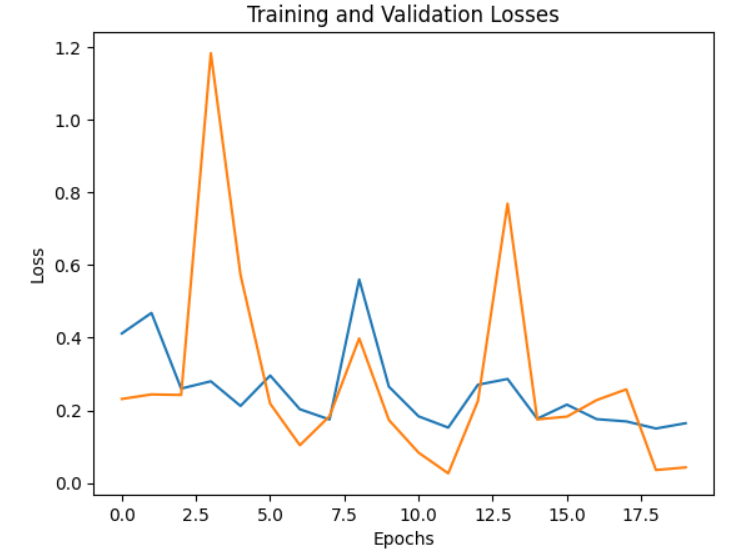
\includegraphics[width=0.75\textwidth]{losses.PNG}
    \caption{Train and Validation Losses}
    \label{fig:my_pic}
\end{figure}


\begin{python}
# Train the model
num_epochs = 20
loss_list = []
train_losses = []
val_losses = []
for epoch in range(num_epochs):
    # Training loop
    mlp_model.train()
    train_loss = 0.0
    for batch_idx, (data, target) in enumerate(train_loader):
        optimizer.zero_grad()
        output = mlp_model(data)
        loss = loss_fn(output, target)
        loss.backward()
        optimizer.step()
        
        train_loss += loss.item()
    train_losses.append(loss.item())
    # Print the epoch and training loss
    print("Epoch [{}/{}], Training Loss: {:.4f}".format(epoch+1, num_epochs, loss.item()))
    
    # Validation loop
    mlp_model.eval()
    val_loss = 0.0
    with torch.no_grad():
        for batch_idx, (data, target) in enumerate(val_loader):
            output = mlp_model(data)
            val_loss += loss_fn(output, target).item() * data.size(0)
    val_loss /= len(val_loader.dataset)
    val_losses.append(val_loss)
    # Print the epoch and validation loss
    print('Epoch [{}/{}], Validation Loss: {:.4f}'.format(epoch+1, num_epochs, val_loss, train_loss))
    loss_list.append(loss.item())
\end{python}



\subsection{(10 Puan)} \textbf{SEED=öğrenci numaranız set ettikten sonra altıncı haftada ödev olarak verdiğim gibi earlystopping'deki en iyi modeli kullanarak, Prensesi İyileştir test setinden accuracy, F1, precision ve recall değerlerini hesaplayan kodu yazın ve sonucu da aşağı yapıştırın. \%80'den fazla başarı bekliyorum test setinden. Daha düşükse başarı oranınız, nerede hata yaptığınızı bulmaya çalışın. \%90'dan fazla başarı almak mümkün (ben denedim).}

\begin{python}
from sklearn.metrics import accuracy_score, confusion_matrix, precision_score, recall_score, f1_score

Z_test = torch.tensor(test_df.iloc[:, :-1].values, dtype=torch.float32)
Q_test = torch.tensor(test_df.iloc[:, -1].values, dtype=torch.float32)

with torch.no_grad():
    mlp_model.eval()
    y_pred = mlp_model(Z_test)
    y_pred_classes = y_pred.argmax(dim=1).cpu().numpy()
    if Q_test.ndim > 1:
        y_true = Q_test.argmax(axis=1)
    else:
        y_true = Q_test

accuracy = accuracy_score(y_true, y_pred_classes)
confusion_mtx = confusion_matrix(y_true, y_pred_classes)
precision = precision_score(y_true, y_pred_classes, average='weighted', zero_division=1)
recall = recall_score(y_true, y_pred_classes, average='weighted', zero_division=1)
f1 = 2 * (precision * recall) / (precision + recall)

print("Confusion Matrix:\n", confusion_mtx)
print("Accuracy: {:.4f}".format(accuracy))
print("Precision: {:.4f}".format(precision))
print("Recall: {:.4f}".format(recall))
print("F1 Score: {:.4f}".format(f1))


\end{python}

Epoch [1/100], Training Loss: 0.6651
.
.
.
.
Epoch [29/100], Training Loss: 0.0048
Early stopping!
Accuracy: 0.4974
Precision: 0.7500
Recall: 0.4974
F1 Score: 0.5981

\subsection{(5 Puan)} \textbf{Tüm kodların CPU'da çalışması ne kadar sürüyor hesaplayın. Sonra to device yöntemini kullanarak modeli ve verileri GPU'ya atıp kodu bir de böyle çalıştırın ve ne kadar sürdüğünü hesaplayın. Süreleri aşağıdaki tabloya koyun. GPU için Google Colab ya da Kaggle'ı kullanabilirsiniz, iki ortam da her hafta saatlerce GPU hakkı veriyor.}

\begin{table}[ht!]
    \centering
    \caption{Çalışma Süreleri}
    \begin{tabular}{c|c}
        CPU & 8.1969 saniye \\
        GPU & 1.3214 saniye\\
    \end{tabular}
    \label{tab:my_table}
\end{table}

\subsection{(3 Puan)} \textbf{Modelin eğitim setine overfit etmesi için elinizden geldiği kadar kodu gereken şekilde değiştirin, validasyon loss'unun açıkça yükselmeye başladığı, training ve validation loss'ları içeren figürü aşağı koyun ve overfit için yaptığınız değişiklikleri aşağı yazın. Overfit, tam bir çanak gibi olmalı ve yükselmeli. Ona göre parametrelerle oynayın.}


\begin{figure}[ht!]
    \centering
    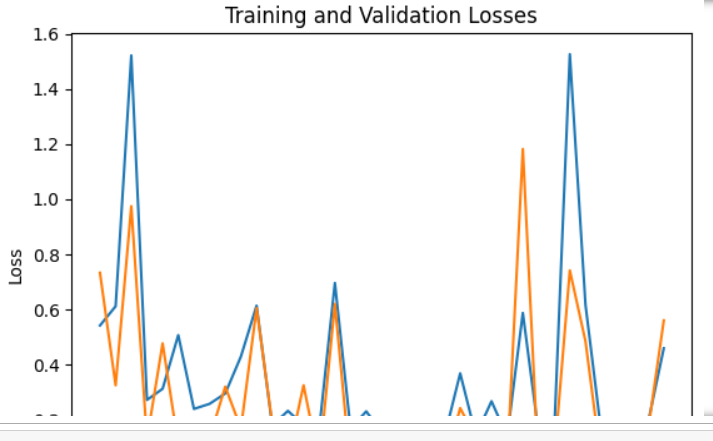
\includegraphics[width=0.75\textwidth]{losses2.PNG}
    \caption{Train and Validation Losses}
    \label{fig:my_pic}
\end{figure}

Modelin overfit etmesi için batch size'ı arttırmayı denedim. Belirgin bir şekilde olmasa da validasyon loss'un arttığını gördüm. Batch size'ı ise sizin derste anlattığınız gibi early stopping noktasını (veriden daha büyük parçalar aldığımız için) aşacağını düşünerek arttırmak aklıma geldi. 



% Figür aşağı
\begin{comment}
\begin{figure}[ht!]
    \centering
    \includegraphics[width=0.75\textwidth]{mypicturehere.png}
    \caption{Buraya açıklama yazın}
    \label{fig:my_pic}
\end{figure}
\end{comment}

\subsection{(2 Puan)} \textbf{Beşinci soruya ait tüm kodların ve cevapların olduğu jupyter notebook'un Github linkini aşağıdaki url'e koyun.}

\url{https://github.com/cngzerms/neuralNetworks_secondStep.git}

\section{(Toplam 10 Puan)} \textbf{Bir önceki sorudaki Prensesi İyileştir problemindeki yapay sinir ağınıza seçtiğiniz herhangi iki farklı regülarizasyon yöntemi ekleyin ve aşağıdaki soruları cevaplayın.} 

\subsection{(2 puan)} \textbf{Kodlarda regülarizasyon eklediğiniz kısımları aşağı koyun:} 

Derste anlattığınız dropout yöntemini kullandım.

\begin{python}
class MLP(nn.Module):
    def __init__(self, input_dim, hidden_dim1, hidden_dim2, output_dim):
        super(MLP, self).__init__()
        self.layer1 = nn.Linear(input_dim, hidden_dim1)
        self.layer2 = nn.Linear(hidden_dim1, hidden_dim2)
        self.output = nn.Linear(hidden_dim2, output_dim)
        self.relu = nn.ReLU()
        self.sigmoid = nn.Sigmoid()
        self.dropout = nn.Dropout(0.15) # DROPOUT
        
    def forward(self, x):
        x = self.layer1(x)
        x = self.relu(x)
        x = self.dropout(x)   #DROPOUT
        x = self.layer2(x)
        x = self.relu(x)
        x = self.dropout(x)   #DROPOUT
        x = self.output(x)
        x = self.sigmoid(x)
        return x
\end{python}

\subsection{(2 puan)} \textbf{Test setinden yeni accuracy, F1, precision ve recall değerlerini hesaplayıp aşağı koyun:}

Test accuracy: 0.0000
Accuracy: 0.4974
Precision: 0.7500
Recall: 0.4974
F1 Score: 0.5981

\subsection{(5 puan)} \textbf{Regülarizasyon yöntemi seçimlerinizin sebeplerini ve sonuçlara etkisini yorumlayın:}

Earlystopping ve dropout yöntemlerini kullandım. Sebebi sadece bunları sizden öğrenmiş olmam farklı yolları aramadım bunlarla yaptım :) . Modelin performansı biraz daha arttı.
Dropout özelliğini eklememle birlikte doğal olarak daha fazla epoch ilerlediğini gördüm. Daha önce 30-40. civarı epoch sırasında earlystopping yaparken dropout'la beraber 70. epoch'a kadar earlystopping yapmadan ilerleyebildi.

Recall ve precision değerlerinin düşük miktar düşmesi beklenir gibi bir bilgi gördüm internette (dropout yönteminin uygulanmasıyla) bende ise bir düşüş göremedim. 

Bunlara ek olarak validation ve training loss'lar grafikte daha girintili çıkıntılı gözüktü. Dropout yönteminde bununda olduğunu göstermiştiniz.

\subsection{(1 puan)} \textbf{Sonucun github linkini  aşağıya koyun:}

\url{https://github.com/cngzerms/neuralNetworks_thirdStep.git}

\end{document}